\documentclass{article}
\usepackage{geometry}
\usepackage{microtype}
\usepackage{enumitem}
\usepackage{graphicx}
\usepackage{floatrow}
\usepackage{caption}

\newlist{mylist}{itemize}{1}
\setlist[mylist]{
  label=\textbf{\{},
  after=\textbf{\}},
  labelsep=0.000001em,
}

\geometry{
  left=1.3cm, 
  right=1.1cm,
  top=1.8cm,
  bottom=2cm 
}

\begin{document}
\begin{minipage}[t]{0.45\textwidth}
    embedding data at lower levels of production, such as production processes and equipment (see [15]). The connection with other software components that solve different tasks (acquiring, saving, displaying, analyzing data, etc.) should also be taken into account, but in general they form a digital twin (see [23]). The P\&ID production scheme serves as the source of this data. Therefore the ISA 5.1 standard [18] has to work with the P\&ID scheme and is widely used in control systems along with the ISA 88 standard to fully describe the lower production levels. This standard is useful when a reference to equipment is required in the chemical, petroleum, power generation, air conditioning, metal refining, and many other industries. The purpose of this standard is to establish a consistent method of naming instruments and instrumentation systems used for measurement and control. For this purpose, a designation system is presented that includes symbols and identification codes.
    
    \hspace{0.2cm} One of the important problems when implementing a standard at a company is the possibility of ambiguous interpretation of various parts of standard, as well as the necessity to constantly alter and improve this interpretation in such a way that it becomes closer to original. Moreover, there are specific features of implementing a standard at a particular company, the necessity to update the standard that is being used (because each standard constantly evolves) followed by changes to structure and organization of the company’s activities to ensure compliance with the standard.

    \hspace{0.2cm} In order to build a mathematical model of a production system it is required to formalize the technological processes of this production system. The formalization of the mathematical models of the object under study and the control contour is based upon the results of authors’ research in the area of simulating modeling of complex technical systems [2].

    \hspace{0.2cm} Traditionally two groups of technological processes are being considered:
\begin{itemize}[noitemsep,topsep=2pt]
\item continuous;
\item descrete.
\end{itemize}
    \vspace{0.1\baselineskip} \hspace{0.2cm} The first group of technological processes is usually implemented during the production in real-time. These technological processes are a subject of an automated control system of a technological process (ACSTP). For example, ACSTP can be used to control the process of steelmaking, control the flow of raw materials into open-hearth furnaces and automatic pouring of metal into molds. The second group of technological processes is characterized by a graph structure of a technological cycle organization, that operates as set of interconnected operations \textit{\{TCO\textsubscript{i}\}}. Some \textit{TCO\textsubscript{i}} may in their turn consist of a set of microtechnological operations \textit{\{MTCO\textsubscript{ij}\}}.

    \hspace{0.2cm} Depending on how \textit{\{TCO\textsubscript{i}\}} include \textit{\{MTCO\textsubscript{ij}\}} the following types of technological processes can be identified:

\end{minipage}
\hspace{0.2cm} 
\begin{minipage}[t]{0.45\textwidth}

\begin{itemize}[noitemsep,topsep=2pt]
\item single-level processes, which consist of \textit{\{MTCO\textsubscript{ij}\}} that can run in parallel or sequentially based on thegraph structure that describes connections between \textit{MTCO\textsubscript{ij}} );
\item hierarchical processes, that feature a main technological branch that is divided into several child-branches, that will then merge again; in this case as part of \textit{MTCO\textsubscript{ij}} of any level there are operations of "splitting" of technological lines and operations of "merging" of technological lines;
\item iterative, that feature child operations nested within the main operations; in this case the operation execution results at some nesting level are used to execute child technological branches.
\end{itemize}
    \vspace{0.2\baselineskip} \hspace{0.2cm} Modeling of all types of technological processes is performed based on critical or average values of resource consumption. Probabilistic technological processes of the second and the third type are considered to be the most difficult to model.

    \hspace{0.2cm} When \textit{MTCO\textsubscript{ij}} is running resources of the technological cycle are being spent. Based on the nature of resource consumption two groups of processes can be considered:
\begin{itemize}[noitemsep,topsep=2pt]
  \item \vspace{0.3\baselineskip} deterministic processes (DTP) that have resources consumed based on critical or average values;
  \item probabilistic processes (PTP) that have some resources consumed in deterministic way (defined by lists of resources and their volumes) while other resources are being spent in a probabilistic way (defined by probability distribution functions for the resource consumption) by its \textit{MTCO\textsubscript{ij}}.
\end{itemize}
    \vspace{0.3\baselineskip} \hspace{0.2cm} Some \textit{MTCO\textsubscript{ij}} of a PTP may not only consume resources during operation but also perform control activities that change control variables \textit{U\textsubscript{s}} of the PTP. 
    
    \hspace{0.2cm} During PTP’s normal opearation each component of the \textit{U\textsubscript{s}} control variables set must be within acceptable ranges of minimal ($U_{\mathit{\scriptsize s}}^{-}$) and maximal ($U_{\mathit{\scriptsize s}}^{+}$) values. These changes in \textit{U\textsubscript{s}} values may also be of probabilistic nature. Some \textit{MTCO\textsubscript{ij}} may alter control variables values in such a way that \textit{U\textsubscript{s}} are returned into acceptable ranges ($U_{\mathit{\scriptsize s}}^{-} \leq \textit{U\textsubscript{s}} \leq U_{\mathit{\scriptsize s}}^{+}$).
    
    \hspace{0.2cm} Let us consider a task of modeling reliability characteristics for the technological cycle hardware.

    \hspace{0.2cm} PTP uses in its operation technological units (machines) that may have various reliability characteristics. The technological units have some resource of operation that would gradually decrease depending on the time of active usage of the given unit. When a hardware unit reaches a threshold for this resource during active operation the probability of failure increases dramatically and therefore in a real world situation it is necessary to act in a timely manner and switch to a reserve unit (if possible) or perform maintenance in order to restore the unit’s resource.
 
\end{minipage}

\newpage

\begin{minipage}[t]{0.45\textwidth}
    The moments of time at which a unit will fail are determined by probability distribution functions for the machine’s operation time before failure. Units’ failures may result in emergencies of different types that require quick reactions in order to eliminate their consequences, which may lead to the expenditure of material resources and time delays.

    \hspace{0.2cm} Reliability characteristics of hardware units are defined the following way [2]:
\begin{itemize}[noitemsep,topsep=2pt]
    \item  moments of hardware failures are defined by the probability distribution function F($\tau$\textit{\textsubscript{NO$\omega$}}) of normal operation for the appropriate unit; when the value is exceeded by the operation time a failure will occur;
    \item if a simple failure happens normal operation can be restored after an interval ($\tau$\textit{\textsubscript{RO$\omega$}}) ;
    \item some failures may lead to a simple emergency with probability (P\textit{\textsubscript{f1}}) ; liquidating an emergency requires ($\tau$\textit{\textsubscript{EM1$\omega$}}) additional time and (\textit{c\textsubscript{EM1$\omega$}}) of additonal costs to cover the restoration of normal operation;
    \item some failures may lead to a complex emergency with probability (P\textit{\textsubscript{f2}}) ; liquidating of such an emergency requires execution of a sequence of special technological operations; each of those operation may require additional time ($\tau$\textit{\textsubscript{liq}}) and additional costs (\textit{c\textsubscript{liq}}) ; therefore liquidation of such a complex emergency may lead to operation time delay of $\sum$$\tau$\textit{\textsubscript{liq}} and increases in costs of $\sum$$\tau$\textit{\textsubscript{liq}} .
\end{itemize}
    \vspace{0.3\baselineskip} \hspace{0.2cm} A separate type of PTP can be considered where emergency may lead to stop of operation for the whole PTP. Such emergences are liquidated as the complex emergences but the whole TP operation halts until the liquidation is finished.

    \hspace{0.2cm} Thus project modeling of the PTP is a complex scientific problem due to the probabilistic nature of the resource consumption by \textit{\{MTCO\textsubscript{ij}\}} and presence of equipment failures that may also be of probabilistic nature.
\begin{center}
    \vspace{0.4\baselineskip} \textsc{V. Formalization of the Technological cycle  control contour based on OSTIS Technology}
\end{center}
    
    \vspace{0.4\baselineskip} \hspace{0.2cm} In line with the knowledge domain ontology for the probabilistic technological processes, the technological production cycle means a sequence of actions and operations that result in some final (or semi-final for this stage) product.

    \hspace{0.2cm} The functional interaction between the components of the control complex and the operating in real-time technological production cycle is based on continuous monitoring of the equipment states and the control parameters through registers indicators and means of technical coupling.

    \hspace{0.2cm} In order to build a robust semantically compatible intellectual system for control adaptation OSTIS Technology will be used as a base for the control complex. The system includes agents to address the tasks of interacting

    
\end{minipage}
\hspace{0.2cm} 
\begin{minipage}[t]{0.45\textwidth}
    with the means of technical coupling and making control decisions.

    \hspace{0.2cm} In OSTIS Technology problem solvers are implemented based on multi-agent approach. According to this approach the solver is constructed as a set of agents, that are called sc-agents. All such agents share memory and may exchange data through special semantic structures (sc-texts). It is important to note  that some agents may not be atomic (i.e. may consist of two or more sc-agents).

    \hspace{0.2cm} The full problems solver for the control task can be implemented as a decomposition of an abstract nonatomic sc-agent.

    \textbf{\textit{abstract non-atomic sc-agent of cycle recommendation system}}

    $\Rightarrow$ \hspace{0.7cm}\textit{decomposition of abstract sc-agent*:}
\begin{mylist}
  \item \begin{itemize} 
    \item \textit{abstract sc agent of interaction with the observation system}
    \item \textit{abstract sc agent of forming recommendations}
    \item \textit{abstract sc-agent of forming requests}
  \end{itemize}
\end{mylist}
    \begin{enumerate}[label={\arabic*)}, noitemsep]
    \item abstract sc-agent of interaction with the observation system — is used to extract observations from the means of hardware-software coupling in the technological cycle; it initiates operation of agent for forming recommendations;
    
    \item abstract sc-agent of forming recommendations — based on the received observations initializes controller operation in order to get recommendation for control actions;
    
    \item abstract sc-agent of forming requests — based on the data received from the agent of forming recommendations forms requests for changing the control cariables of the PTP through the appropriate hardware-software means of coupling.
    \end{enumerate}
    \vspace*{-0.8em}
    \hspace{0.2cm} Agents of interaction with the observation system and forming requests must correspond with the technical communicating with the means of technical coupling.

    \hspace{0.2cm} When developing a control adaptation system within the task of building an ostis-system solver of the given structure an agent for forming recommendations based on the received observations must be created.

    \hspace{0.2cm} Construction of the controller used by the sc-agent of forming recommendations can be based on neural networks as well as other modern machine learning models and algorithms.
    \begin{center}
    \textsc{VI. Developing neuroregulator models for adaptive control problems}
    \end{center}
    \hspace{0.2cm} Several approaches may be proposed when considering the adaptive control problem:

 \begin{enumerate}[label={\arabic*)}, noitemsep]
    \item direct control (controller modeling), when a neural network is trained on a database of existing optimal
 \end{enumerate}

\end{minipage}

\newpage

\begin{minipage}[t]{0.45\textwidth}
\begin{enumerate}[label={\arabic*)}, start=2,  noitemsep]
    \item[] signals (of an existing controller) [5] that lead to the desired trajectories in the phase space of the system and thus the neurocontroller for the control system is built [12]. Such a scheme is one of the most simple ones, but it has flaws such as a requirement to have a representative set of the existing physical controller statistics;

    \item direct inverse control [4], in this case during modeling of the control contour operation the neurocontroller learns to reproduce a relation between the control signal at the current moment of time and observations of the control object at the next moment of time [6] [7];

    \item Schemes may be proposed where the neurocontroller is built using reinforcement learning, particularly:

\begin{itemize}[noitemsep,topsep=2pt]
    \item neurocontroller trained through reinforcement learning procedure for a task of finding an optimal trajectory (optimal in some "geometrical" sense) in the phase space of the control system states [3] [4] [9];
    \item neurocontroller trained through reinforcement learning procedure for a task of implicit optimal trajectory search when some estimation of the control quality \textit{R} is used [10] [11].
\end{itemize}
\end{enumerate}

    \vspace*{-0.8em} Since the problem of selecting an appropriate neural network structure for the particular task is in each case complex and difficult to formalize, it may be useful to consider application of the evolutional methods for its automation. [14] .

    \hspace{0.2cm} When controller modeling is used the neurocontroller is trained in such a way that it would be able to reasonably generalize over the collected data of the control process for the technological cycle. In this case from the machine learning theory point of view, supervised learning occurs, when the collected data will be used as pairs of desired input and output (control signals) vectors of the controller. From the point of view of the dynamical systems theory a phase space of the technological process control system is an environment where a decision about control actions must be made based on the observed state. And therefore the process of neural network training may be viewed as a process of learning the correct trajectories in the phase space that correspond to optimal controls.

\begin{figure}[H]
\centering
\begin{minipage}[t]{0.4\textwidth}
  \centering
  \hspace*{-2.4cm}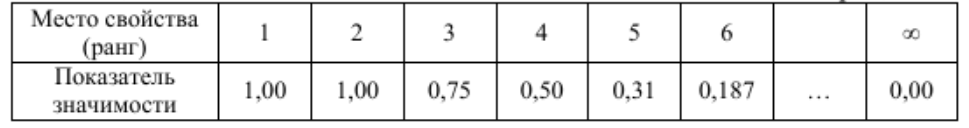
\includegraphics[width=2.4\textwidth]{tab2.png}
  \captionsetup{justification=centering, font=small}
  \caption{Direct control scheme}\label{fig:myfigure}
\end{minipage}%
\end{figure}

    \hspace{0.2cm} Training process with inverse scheme is similar from the machine learning point of view. The difference is that the desired observation signals of the control object are used as a source for building the loss function that would be optimized.

\end{minipage}
\hspace{0.2cm} 
\begin{minipage}[t]{0.45\textwidth}
\begin{figure}[H]
\centering
\begin{minipage}[t]{0.4\textwidth}
  \centering
  \hspace*{-2.4cm}\includegraphics[width=2.4\textwidth]{tab1.png}
  \captionsetup{justification=centering, font=small}
  \caption{An example of a scheme with inverse control}\label{fig:myfigure}
\end{minipage}
\end{figure}

    \vspace{0.4\baselineskip}\hspace{0.2cm} The schemes where reinforcement learning is implemented have a potential for building an effective controller due to the presence of an exploratory element in them when searching for a control strategy. This may have a positive effect when solving problems with complex structure of the control decisions.
\vspace{0.8\baselineskip}
\begin{figure}[H]
\centering
\begin{minipage}[t]{0.4\textwidth}
  \centering
  \hspace*{-2.4cm}\includegraphics[width=2.4\textwidth]{tab3.png}
  \captionsetup{justification=centering, font=small}
  \caption{Reinforcement learning scheme}\label{fig:myfigure}
\end{minipage}%
\end{figure}

    \vspace{0.4\baselineskip}\hspace{0.2cm} Let us consider some functional \textit{R} for estimating the quality of the control (estimation of the quality of the control policy ( cotrol actions selection by agent (control system)) $\pi$ ) that is calculated during the time period of the TP operation [0,\textit{t}]. (For example this functional may "reward" for lowering the production costs and "penalize" for equipment downtime, occurence of hardware failures or emergencies).

    \hspace{0.2cm} Decision making in this case can be managed by a neural network (agent operating under the neural network control).

    \hspace{0.2cm} When agent performs certain actions this leads to some sort of trajectory being built in the phase space (in this context the control construction is considered to be a trajectory construction in the phase space of the technological process control system states).

    \hspace{0.2cm} The problem of search for an optimal trajectory in the phase space of the system, thus is equivalent to maximizing \textit{R} (at this moment of time and at the future moments - meaning that the controller for the technological cycle is required to produce such an action selection policy $\pi$, that would maximize the estimate for control quality \textit{R}).

    \hspace{0.2cm} Application of reinforcement learning methods assumes the existence of environment, in which a critical evaluation of agent’s actions happens. An environment in which an agent operates in the context of the technological cycle control is the system of control of technological production cycle. This environment makes it available for agent’s observations signals of registers indicating

\end{minipage}
\end{document}
